%%% Beamer slideshow
\documentclass[aspectratio=169]{beamer}

\usepackage{natbib,amsmath,amssymb,graphicx}
\usepackage{booktabs}
\usepackage{multirow}
\usepackage{multicol}
\usepackage{array}
\usepackage{bbm}
\usepackage{bm}

\newcolumntype{L}[1]{>{\raggedright\arraybackslash}p{#1}}
\newcolumntype{C}[1]{>{\centering\arraybackslash}p{#1}}
\newcolumntype{R}[1]{>{\raggedleft\arraybackslash}p{#1}}

\graphicspath{{../Figures/Figures_v3/}{../Figures/Figures_Retirement/}{../Figures/DurableModel/}}

\newcommand{\Ret}{\mathrm{Ret}}
\newcommand{\eff}{\varepsilon}
\newcommand{\goth}[1]{\mathcal{#1}}
\newcommand{\E}{\mathbb{E}}

\mode<presentation>
{
	\usetheme{CambridgeUS}
	\usecolortheme{default}
	\usefonttheme{default}
	\setbeamertemplate{navigation symbols}{}
	\mode<beamer>{\setbeamertemplate{blocks}[rounded][shadow=true]}
	\setbeamertemplate{caption}[numbered]
	% miniframes (headline) before infolines (footline); reverse order breaks total frame count
	\useoutertheme[subsection=false]{miniframes}
	\useoutertheme{infolines}
	\setbeamertemplate{page number in head/foot}[totalframenumber]
}

\title[DCEGM Search --- Updates]{Search Smooths Discontinuities:\\ Updates}
\author[Carroll et al.]{Christopher D.\ Carroll\inst{1}, Fedor Iskhakov\inst{2}, Shujaat Khan\inst{3}, and Adrian Monninger\inst{4}}
\institute[]{
	\inst{1}Johns Hopkins University
	\and
	\inst{2}Stony Brook University
	\and
	\inst{3}IMF
	\and
	\inst{4}Texas A\&M University
}
\date{September 18, 2026}

\begin{document}

%%% Title slide
\begin{frame}[plain]
	\titlepage
\end{frame}


%============================================================
\section{Previous story}
%============================================================

%%% Previous story
% Goal: Show Search can smooth discontinuities instead of EV taste shocks
\begin{frame}[label = PrevGoal]
	\frametitle{Previous story: Goal}
	\textbf{Goal:} show that directed search can smooth discontinuities in DC-EGM problems\\ --- as an alternative to EV Type~I taste shocks
	\vspace{1em}
	\begin{itemize}\setlength\itemsep{0.75em}
		\item Standard fix (Iskhakov et al.\ 2017): EV taste shocks randomize the discrete outcome
		\item Search: agents choose effort $\varepsilon_t\in[0,1]$ that raises the probability of switching
		\item Smoothness is part of the agent's economic problem, not only a numerical trick
	\end{itemize}
	\vspace{1em}
	{\small Application: consumption--saving retirement model (work vs retire)}
\end{frame}

% Problem: Not enough smoothing alone
\begin{frame}[label = PrevProblem]
	\frametitle{Previous story: search alone is not enough}
	\begin{itemize}
		\item Search smooths only to the \emph{right} of discontinuities
		\item Low-$M$ workers optimally set $\eff^\ast=0$ (plan to keep working)
		\item[$\Rightarrow$] Asymmetric / one-sided smoothness
	\end{itemize}
	\vspace{-0.35em}
	\begin{center}
		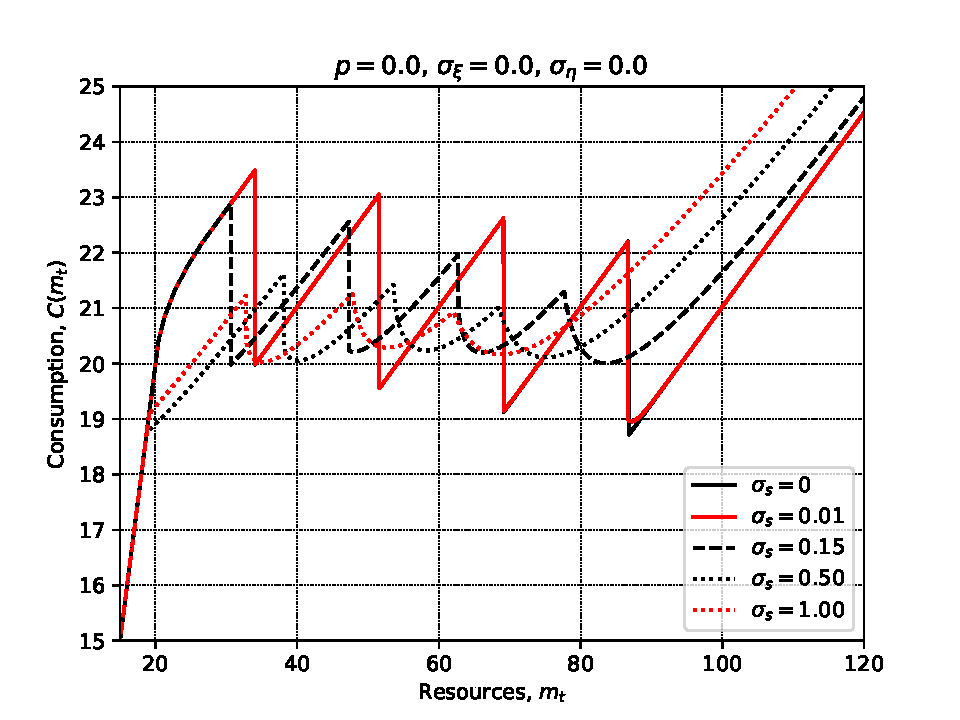
\includegraphics[width=0.4\linewidth]{p0_xi0_eta0.pdf}\\
		{\scriptsize $p=0$: smooths right of kinks}
	\end{center}
\end{frame}

% Solution ideas: combine with taste shocks, exogeneous probability, and income shocks
\begin{frame}[label = PrevIdeas]
	\frametitle{Previous story: candidate complements to search}
	To get uniform smoothness around discontinuities, combine search with:
	\begin{enumerate}\setlength\itemsep{1em}
		\item \textbf{Taste shocks} $\sigma_\xi$ (multiplicative log-normal on the value of working no EV)
		\item \textbf{Exogenous option probability} $p$ (probability of receiving the option without effort)
		\item \textbf{Income shocks} $\sigma_\eta$ (transitory income risk)
	\end{enumerate}
	\vspace{1em}
	{\small All three appear in the retirement application of the paper.}
\end{frame}

% Solution: Search and taste shocks + income shocks smooth it
\begin{frame}[label = PrevSolution]
	\frametitle{Previous story: search + taste (+ income) delivers smoothness}
    \vspace{-1em}
	\begin{columns}[T]
		\begin{column}{0.48\textwidth}
			\centering
			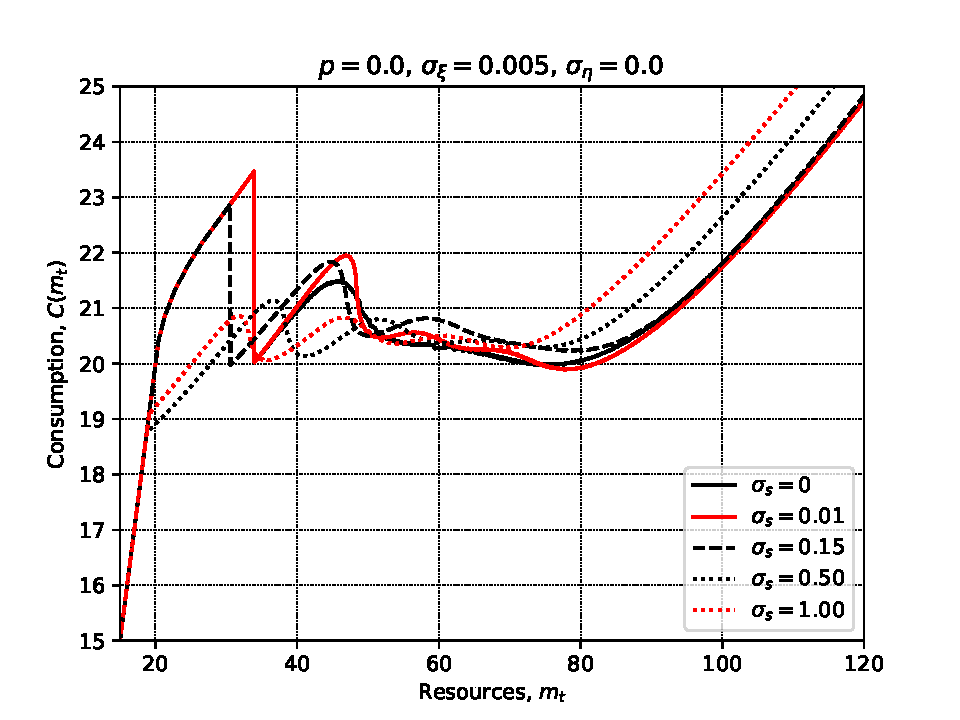
\includegraphics[width=\linewidth]{p0_xi0p005_eta0.pdf}\\
			{\scriptsize Small taste: $\sigma_\xi=0.005$}
		\end{column}
		\begin{column}{0.48\textwidth}
			\centering
			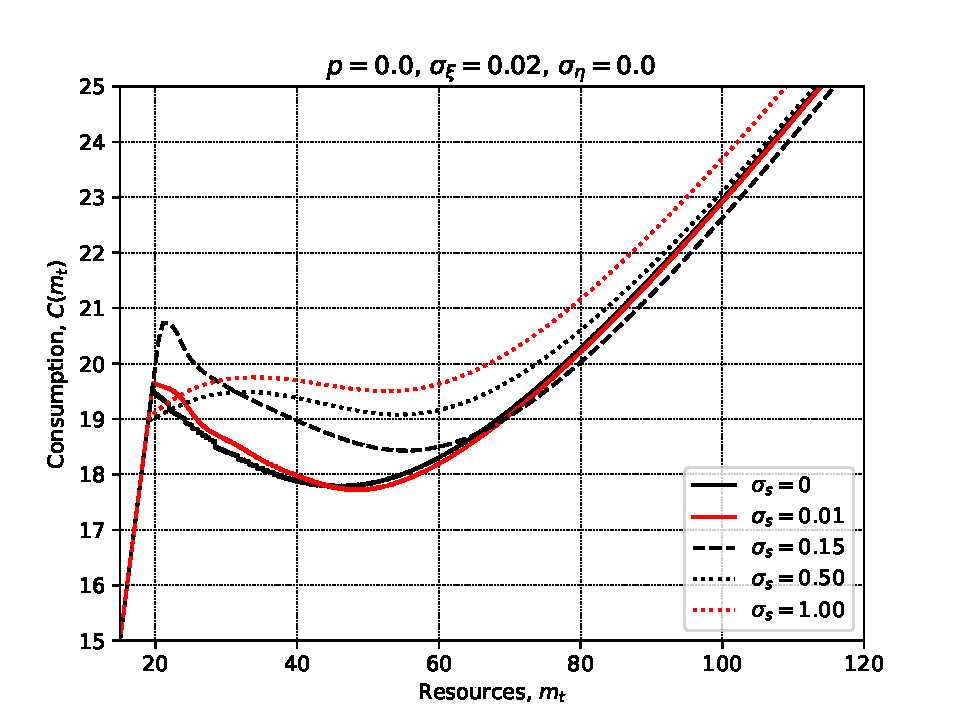
\includegraphics[width=\linewidth]{p0_xi0p02_eta0.pdf}\\
			{\scriptsize Larger taste: $\sigma_\xi=0.02$}
		\end{column}
	\end{columns}
	\vspace{0.5em}
	\begin{itemize}
		\item Taste expands the region where agents search around kinks
		\item With moderate $\sigma_s$ and $\sigma_\xi$, discontinuities are largely smoothed
		\item Income risk adds curvature but does not dominate kink reduction
	\end{itemize}
\end{frame}

% Key insight: Search and taste shocks have opposite effects!
\begin{frame}[label = PrevInsight]
	\frametitle{Key insight: search and taste shift $c$ in opposite directions}
    \vspace{-1em}
	\begin{columns}[T]
		\begin{column}{0.48\textwidth}
			\centering
			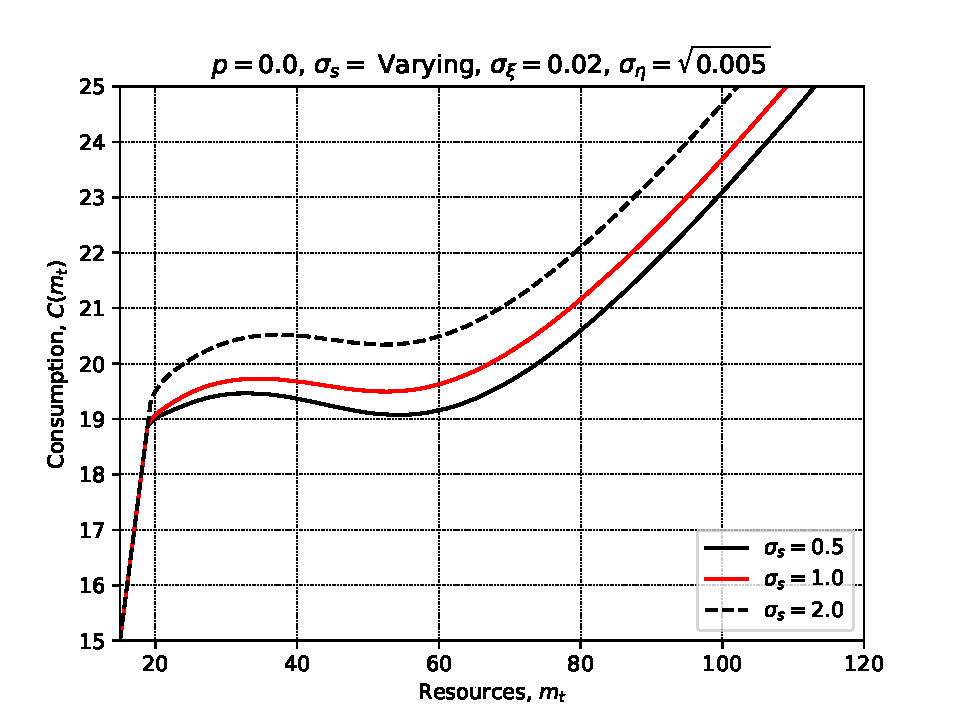
\includegraphics[width=\linewidth]{VaryS.pdf}\\
			{\scriptsize Raising $\sigma_s$ shifts $c$ \textbf{up}}
		\end{column}
		\begin{column}{0.48\textwidth}
			\centering
			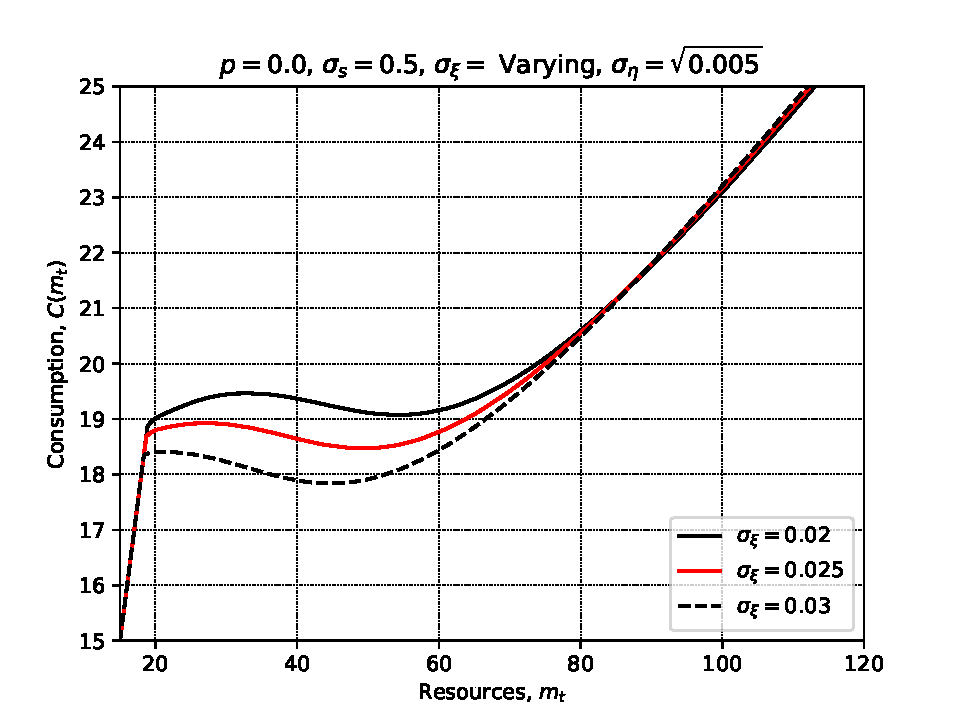
\includegraphics[width=\linewidth]{VaryXi.pdf}\\
			{\scriptsize Raising $\sigma_\xi$ shifts $c$ \textbf{down}}
		\end{column}
	\end{columns}
	\vspace{0.5em}
	\begin{itemize}
		\item Search: utility cost of search $\Rightarrow$ counterbalance with higher $c$
		\item Larger taste shocks: risk of early retirement: $\Rightarrow$ higher savings $\Rightarrow$ lower $c$
	\end{itemize}
\end{frame}


%============================================================
\section{Update 1: Price dispersion}
%============================================================

%%% First update:
% Introduce price dispersion
\begin{frame}[label = Update1Intro]
	\frametitle{Update 1: introduce price / account dispersion}
	\textbf{Idea:} contingent on receiving the option, draw a rejectable realization and then accept or deny
	\vspace{0.75em}
	\begin{itemize}\setlength\itemsep{0.65em}
		\item Retirement: stochastic account factor $\phi_t$ with $\tilde M_t=\phi_t M_t$
		\item Durables: stochastic purchase price $p_t$ on new durable units
		\item Low draw accepted, high draw rejected $\Rightarrow$ softens the extensive margin
	\end{itemize}
	\vspace{0.75em}
	\begin{align*}
		V_t(M_t,\phi_t)=\max\big\{V_t^{\Ret}(\phi_t M_t),\,V_t^{W}(M_t)\big\},\quad
		\bar V_t=\E_{\phi}[V_t]
	\end{align*}
\end{frame}

\begin{frame}[label = Update1PriceAlone]
	\frametitle{Update 1: smoothing through price dispersion}
	\begin{columns}[T]
		\begin{column}{0.48\textwidth}
			\centering
			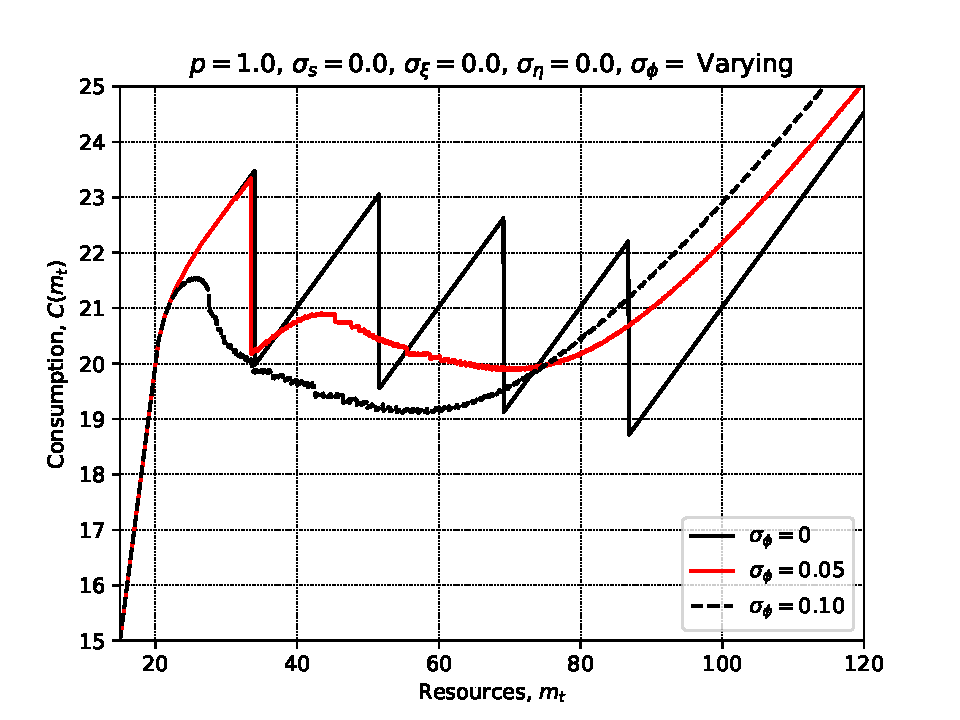
\includegraphics[width=\linewidth]{VaryPhi.pdf}\\
			{\scriptsize Larger $\sigma_\phi$ smooths more}
		\end{column}
		\begin{column}{0.48\textwidth}
			\centering
			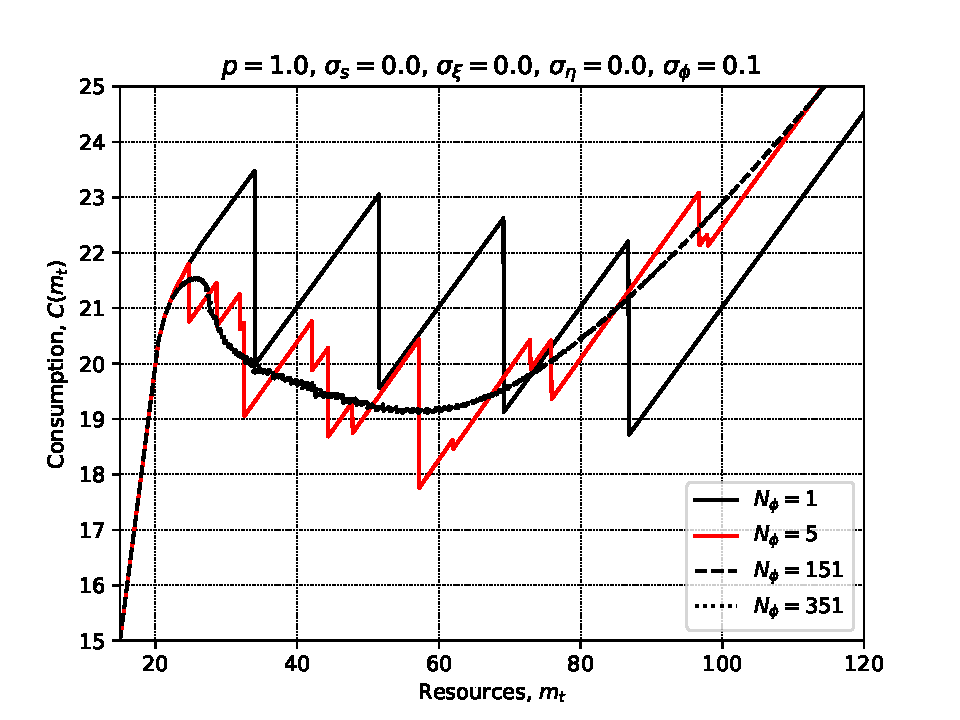
\includegraphics[width=\linewidth]{VaryPhiCount.pdf}\\
			{\scriptsize Need enough $\phi$-nodes}
		\end{column}
	\end{columns}
\end{frame}

% Key insight: Combination of seach and price works great!
\begin{frame}[label = Update1Insight]
	\frametitle{Key insight: search + price dispersion deliver smoothness}
	\begin{itemize}
		\item Search governs \emph{whether} a draw arrives; $\phi_t$ / $p_t$ is the \emph{content} of the draw
		\item Complements: option value of the draw raises search effort
	\end{itemize}
	\vspace{0.35em}
	\begin{columns}[T]
		\begin{column}{0.48\textwidth}
			\centering
			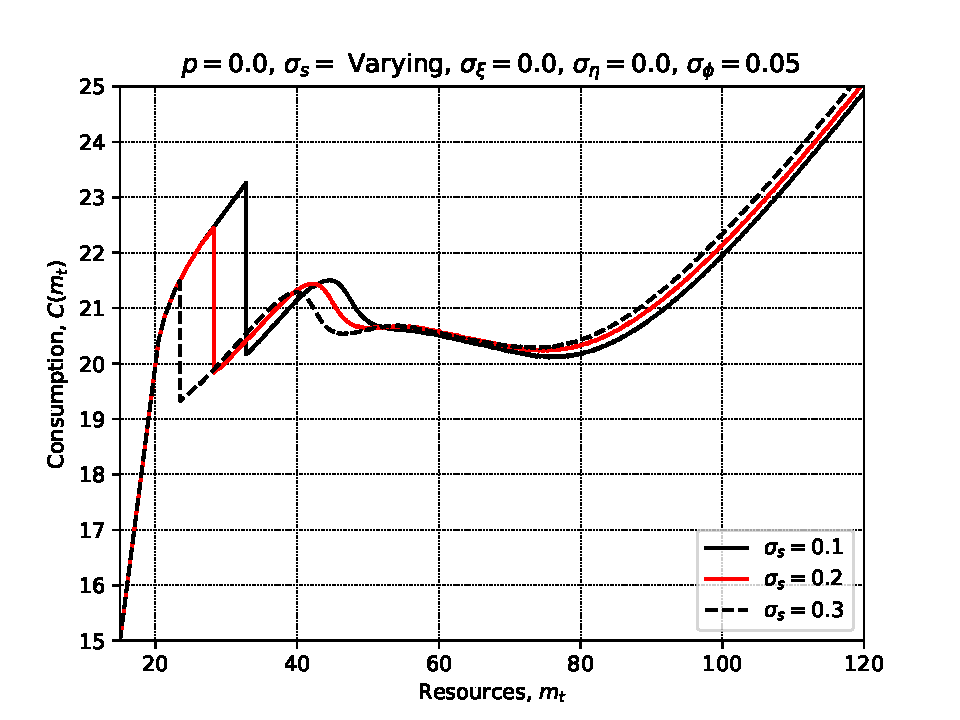
\includegraphics[width=\linewidth]{SearchPhi_VaryS.pdf}\\
			{\scriptsize Vary search given $\phi$}
		\end{column}
		\begin{column}{0.48\textwidth}
			\centering
			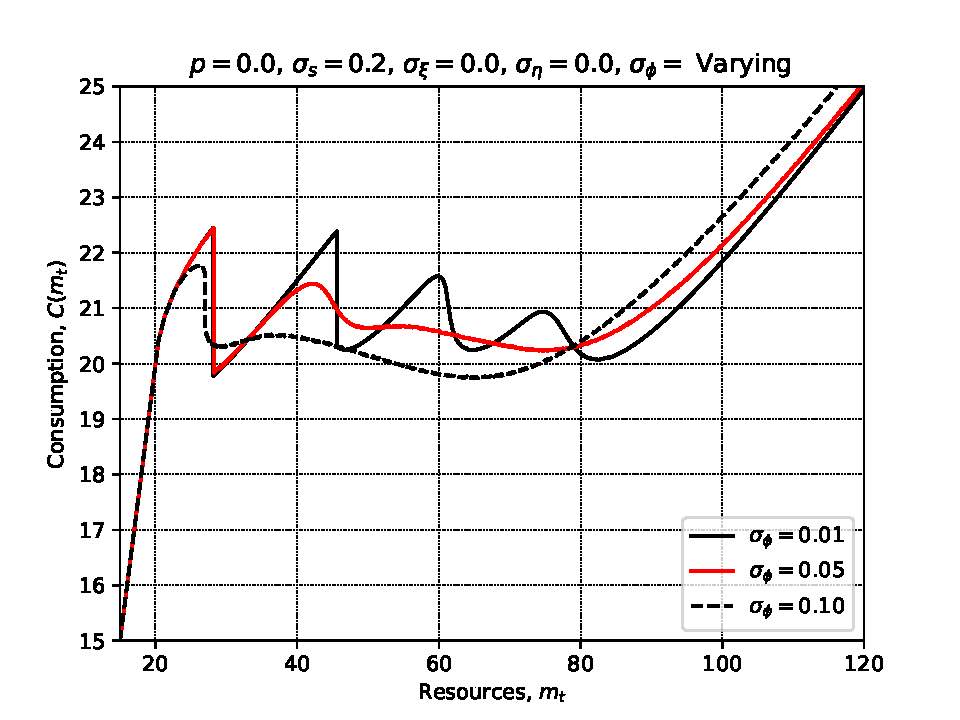
\includegraphics[width=\linewidth]{SearchPhi_VaryPhi.pdf}\\
			{\scriptsize Vary $\sigma_\phi$ given search}
		\end{column}
	\end{columns}
\end{frame}


%============================================================
\section{Update 2: Durable model}
%============================================================

%%% Second update:
% Durable model
\begin{frame}[label = Update2Setup]
	\frametitle{Update 2: durable keep--vs--adjust model in T}
	\begin{itemize}\setlength\itemsep{0.65em}
		\item Discrete choice: keep $d_t=n_t$ vs adjust at cost $\tau$ with liquidity $\ell_t=m_t+(1-\tau)n_t$
		\item Three smoothers: EV taste $\sigma_\varepsilon$, directed search $S$, price dispersion $\sigma_p$
		\item Hard max $\Rightarrow$ S,s bands and discontinuous policies; smoothers soften the band
	\end{itemize}
	\vspace{0.5em}
	\begin{columns}[T]
		\begin{column}{0.32\textwidth}
			\centering
			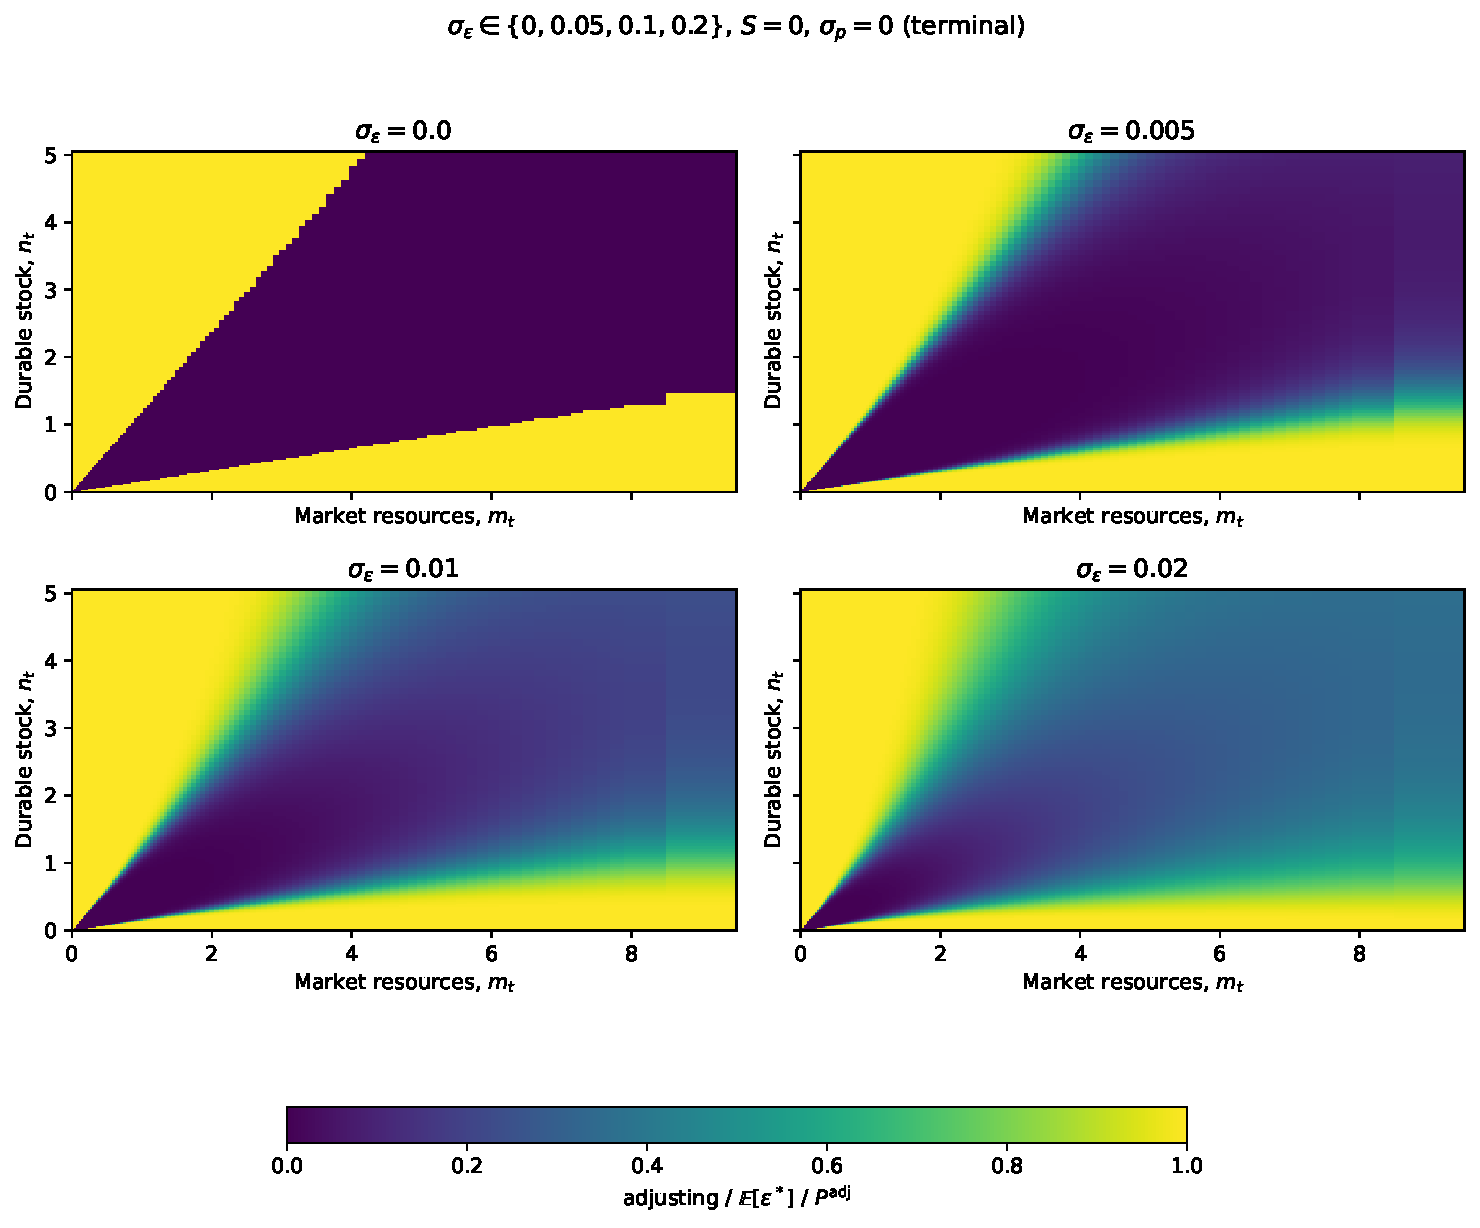
\includegraphics[width=\linewidth]{TasteShock_Ss_T.pdf}\\
			{\scriptsize Taste}
		\end{column}
		\begin{column}{0.32\textwidth}
			\centering
			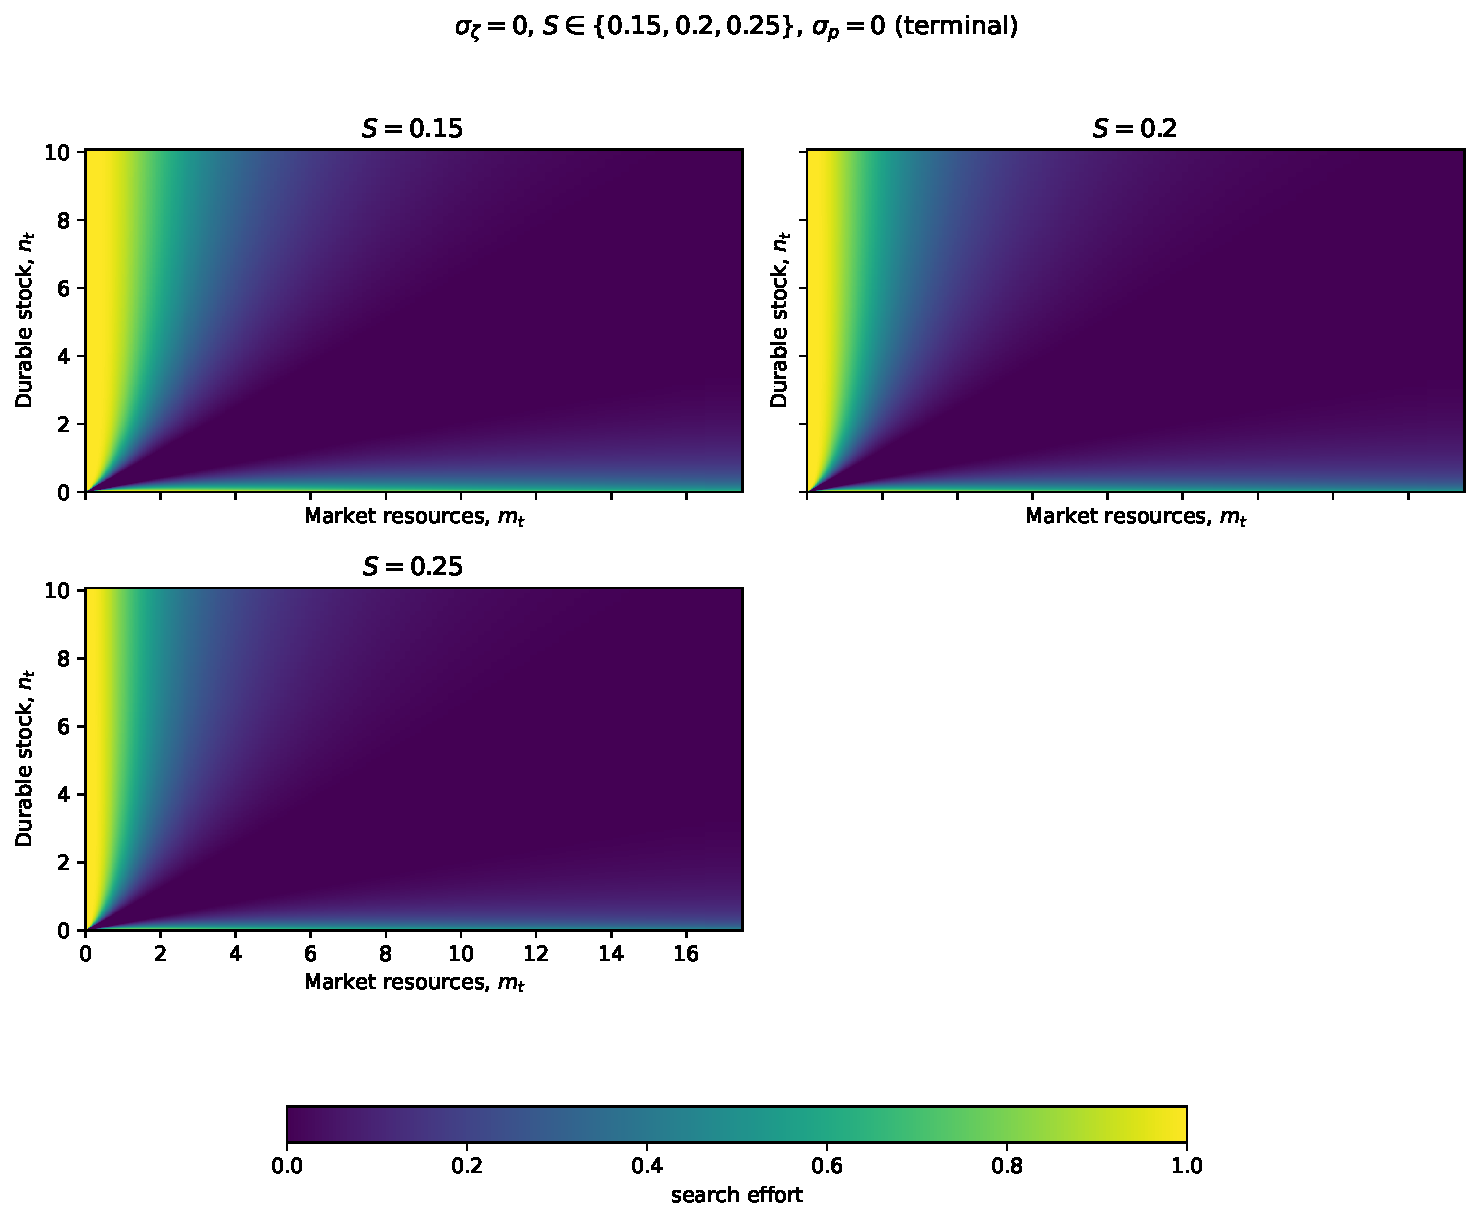
\includegraphics[width=\linewidth]{Search_Ss_T.pdf}\\
			{\scriptsize Search}
		\end{column}
		\begin{column}{0.32\textwidth}
			\centering
			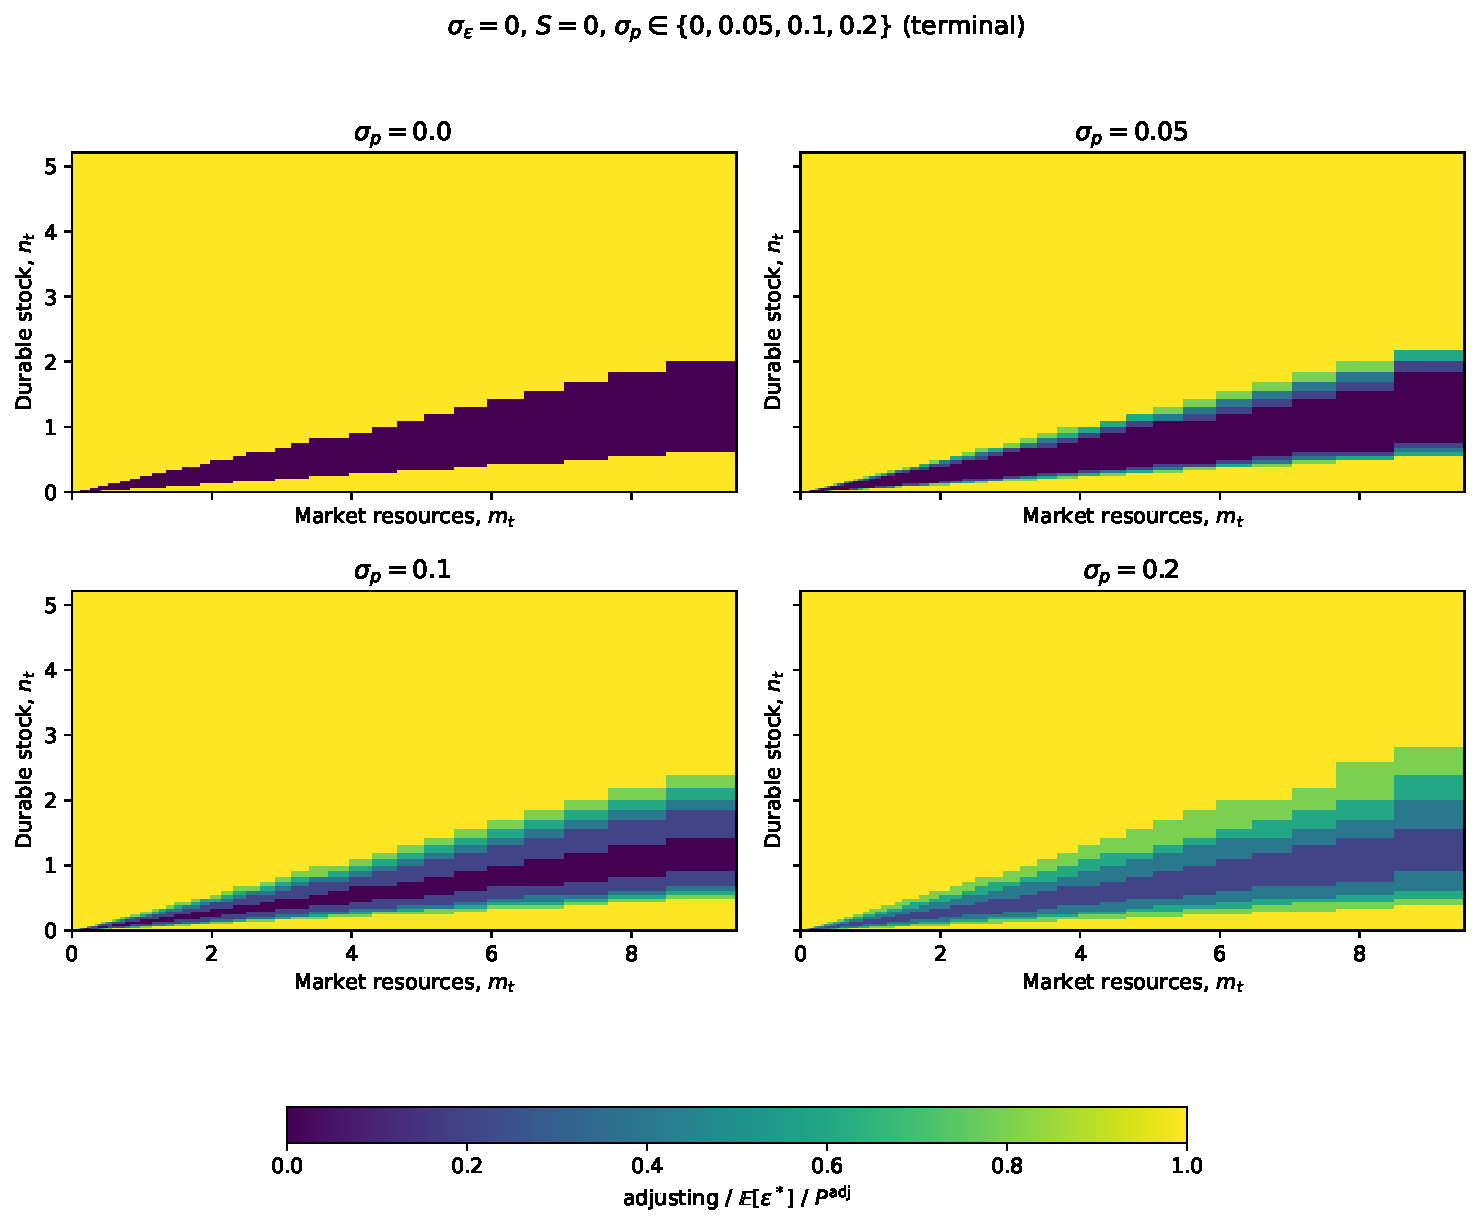
\includegraphics[width=\linewidth]{PriceStd_Ss_T.pdf}\\
			{\scriptsize Prices}
		\end{column}
	\end{columns}
\end{frame}

% \begin{frame}[label = Update2Policies]
% 	\frametitle{Update 2: lifecycle policies --- all channels move together}
% 	\begin{center}
% 		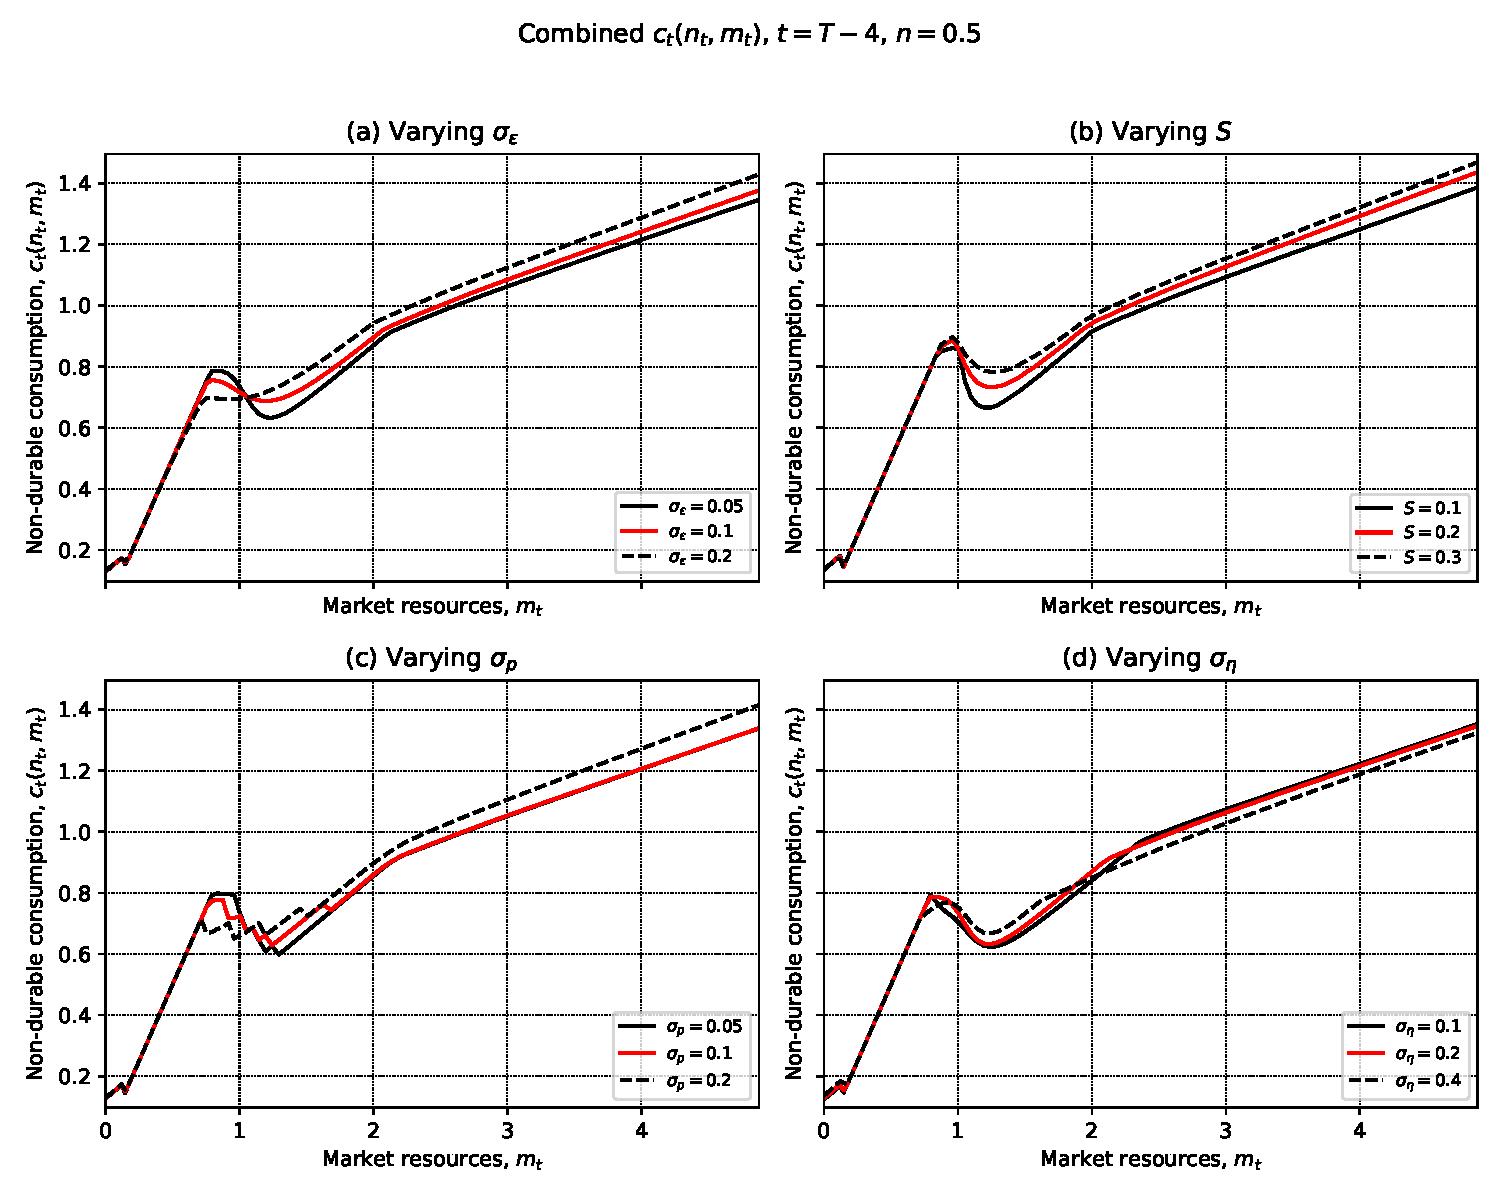
\includegraphics[width=0.5\linewidth]{SmoothingShifts_c_periodt.pdf}
% 	\end{center}
% 	\vspace{-0.15em}
% 	\begin{itemize}
% 		\item Raising $\sigma_\varepsilon$, $S$, $\sigma_p$, or $\sigma_\eta$ raises combined $c_t$ and lowers $d_t$
% 		\item Contrast with retirement: there taste and search shift $c$ in \emph{opposite} directions
% 		\item Here all reweight keep vs adjust toward less aggressive adjustment
% 	\end{itemize}
% \end{frame}

% Key insight 1: all 3 smooth, but have opposite SS effects
\begin{frame}[label = Update2SS]
	\frametitle{Key insight: all three smooth; SS effects diverge}
	\vspace{-0.4em}
	{\footnotesize
	\begin{tabular}{llcccccc}
\hline
 &  & \multicolumn{6}{c}{Steady state} \\
\cline{3-8}
 &  & $C$ & $D$ & $\mathrm{DEX}$ & $\mathrm{TEX}$ & $A$ & $\mathrm{ADJ}$ (\%) \\
\hline
\multirow{3}{*}{$\sigma_\zeta$} & $0.1$ & $0.80$ & $3.56$ & $0.18$ & $0.97$ & $0.94$ & $12.2$ \\
 & $0.15$ & $0.79$ & $3.27$ & $0.16$ & $0.95$ & $0.71$ & $18.6$ \\
 & $0.2$ & $0.79$ & $3.03$ & $0.15$ & $0.94$ & $0.60$ & $24.7$ \\
\addlinespace
\multirow{3}{*}{$\sigma_p$ ($S=0.2$)} & $0.08$ & $0.81$ & $4.28$ & $0.21$ & $1.03$ & $1.39$ & $7.7$ \\
 & $0.1$ & $0.81$ & $4.51$ & $0.23$ & $1.04$ & $1.32$ & $8.7$ \\
 & $0.12$ & $0.82$ & $4.87$ & $0.24$ & $1.06$ & $1.27$ & $9.9$ \\
\addlinespace
\multirow{3}{*}{$S$ ($\sigma_p=0.1$)} & $0.15$ & $0.81$ & $4.59$ & $0.23$ & $1.04$ & $1.27$ & $9.3$ \\
 & $0.2$ & $0.81$ & $4.51$ & $0.23$ & $1.04$ & $1.32$ & $8.7$ \\
 & $0.25$ & $0.81$ & $4.45$ & $0.22$ & $1.04$ & $1.37$ & $8.3$ \\
\hline
\end{tabular}

	}
	\vspace{0.35em}
	\begin{itemize}\setlength\itemsep{0.25em}
		\item{\scriptsize Taste $\uparrow$: More people exogeneously adjust: Adjusting probability $\uparrow$, D $\downarrow$, A $\downarrow$}
        \item{\scriptsize Price dispersion $\uparrow$: Better potential deals: Adjusting probability $\uparrow$, D $\uparrow$, A $\downarrow$}
        \item{\scriptsize Search $\uparrow$: Adjusting becomes more costly: Adjusting probability $\downarrow$, D $\downarrow$, A $\uparrow$}
	\end{itemize}
\end{frame}

% Key insight 1: all 3 smooth, but have opposite SS Jacobian effects
\begin{frame}[label = Update2JacTaste]
	\frametitle{Jacobians: taste changes iMPC impact \emph{and} shape}
	\begin{center}
		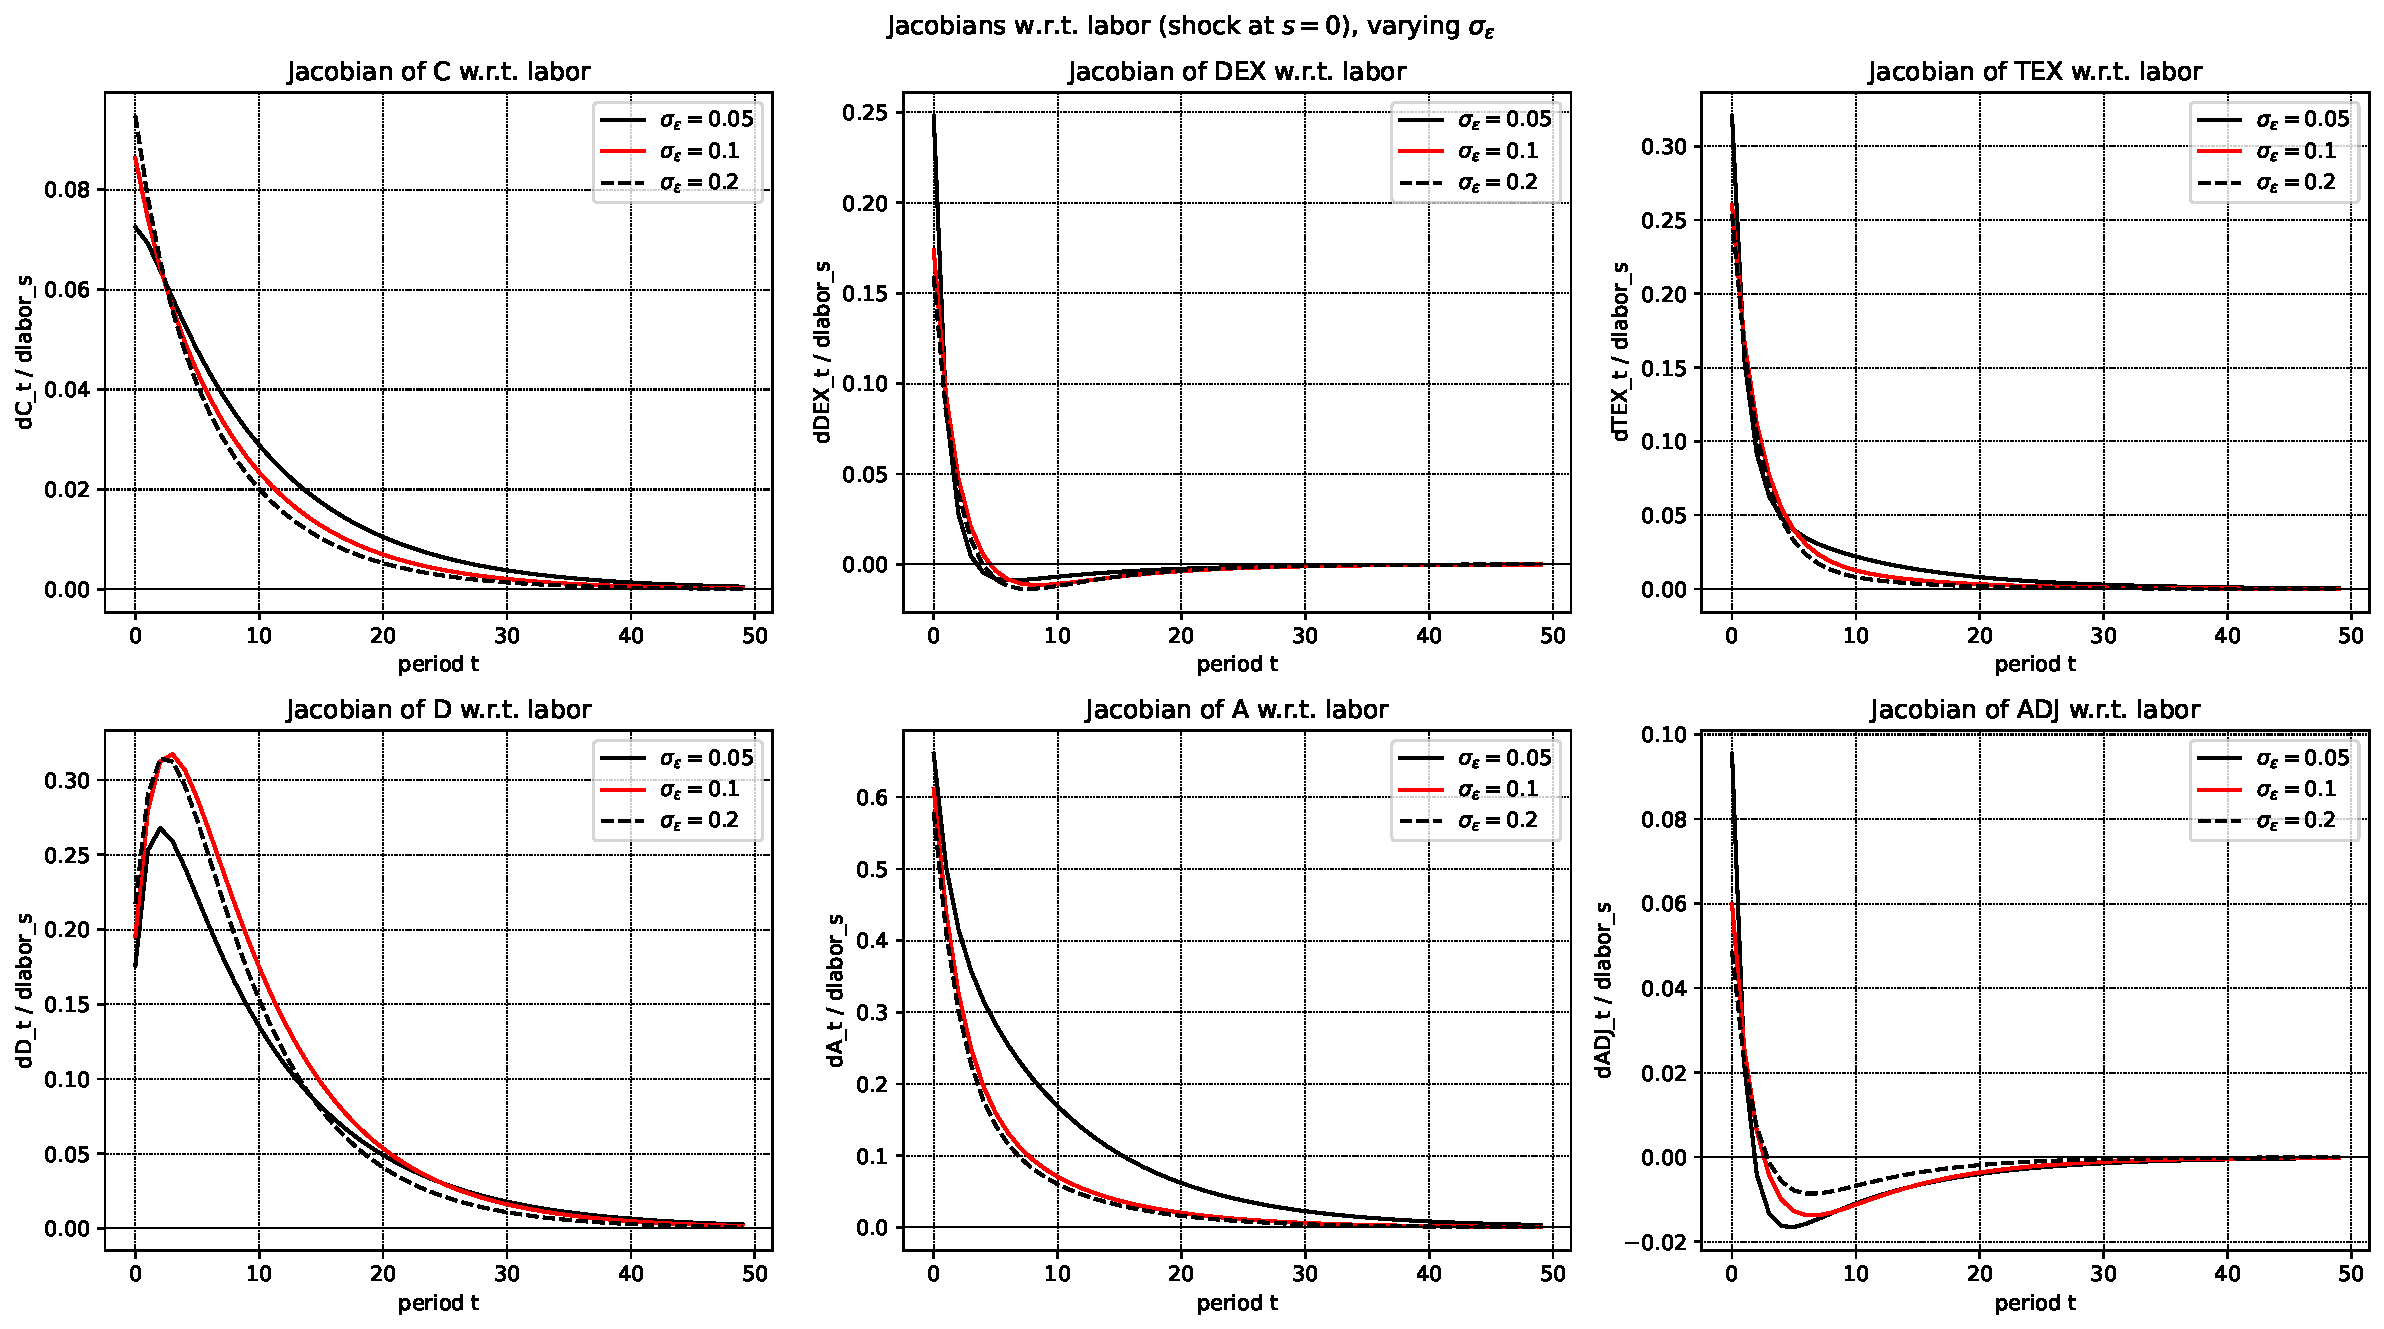
\includegraphics[width=0.78\linewidth]{Taste_Inf_Jacobians_labor.pdf}
	\end{center}
	\vspace{0.25em}
	\begin{itemize}
		\item Sequence-space Jacobians w.r.t.\ labor (fake-news)
		\item Raising $\sigma_\varepsilon$ changes both the \textbf{impact} response and the \textbf{shape} of the Jacobian
	\end{itemize}
\end{frame}

\begin{frame}[label = Update2JacSearch]
	\frametitle{Jacobians: search changes shape, MPC stays the same}
	\begin{center}
		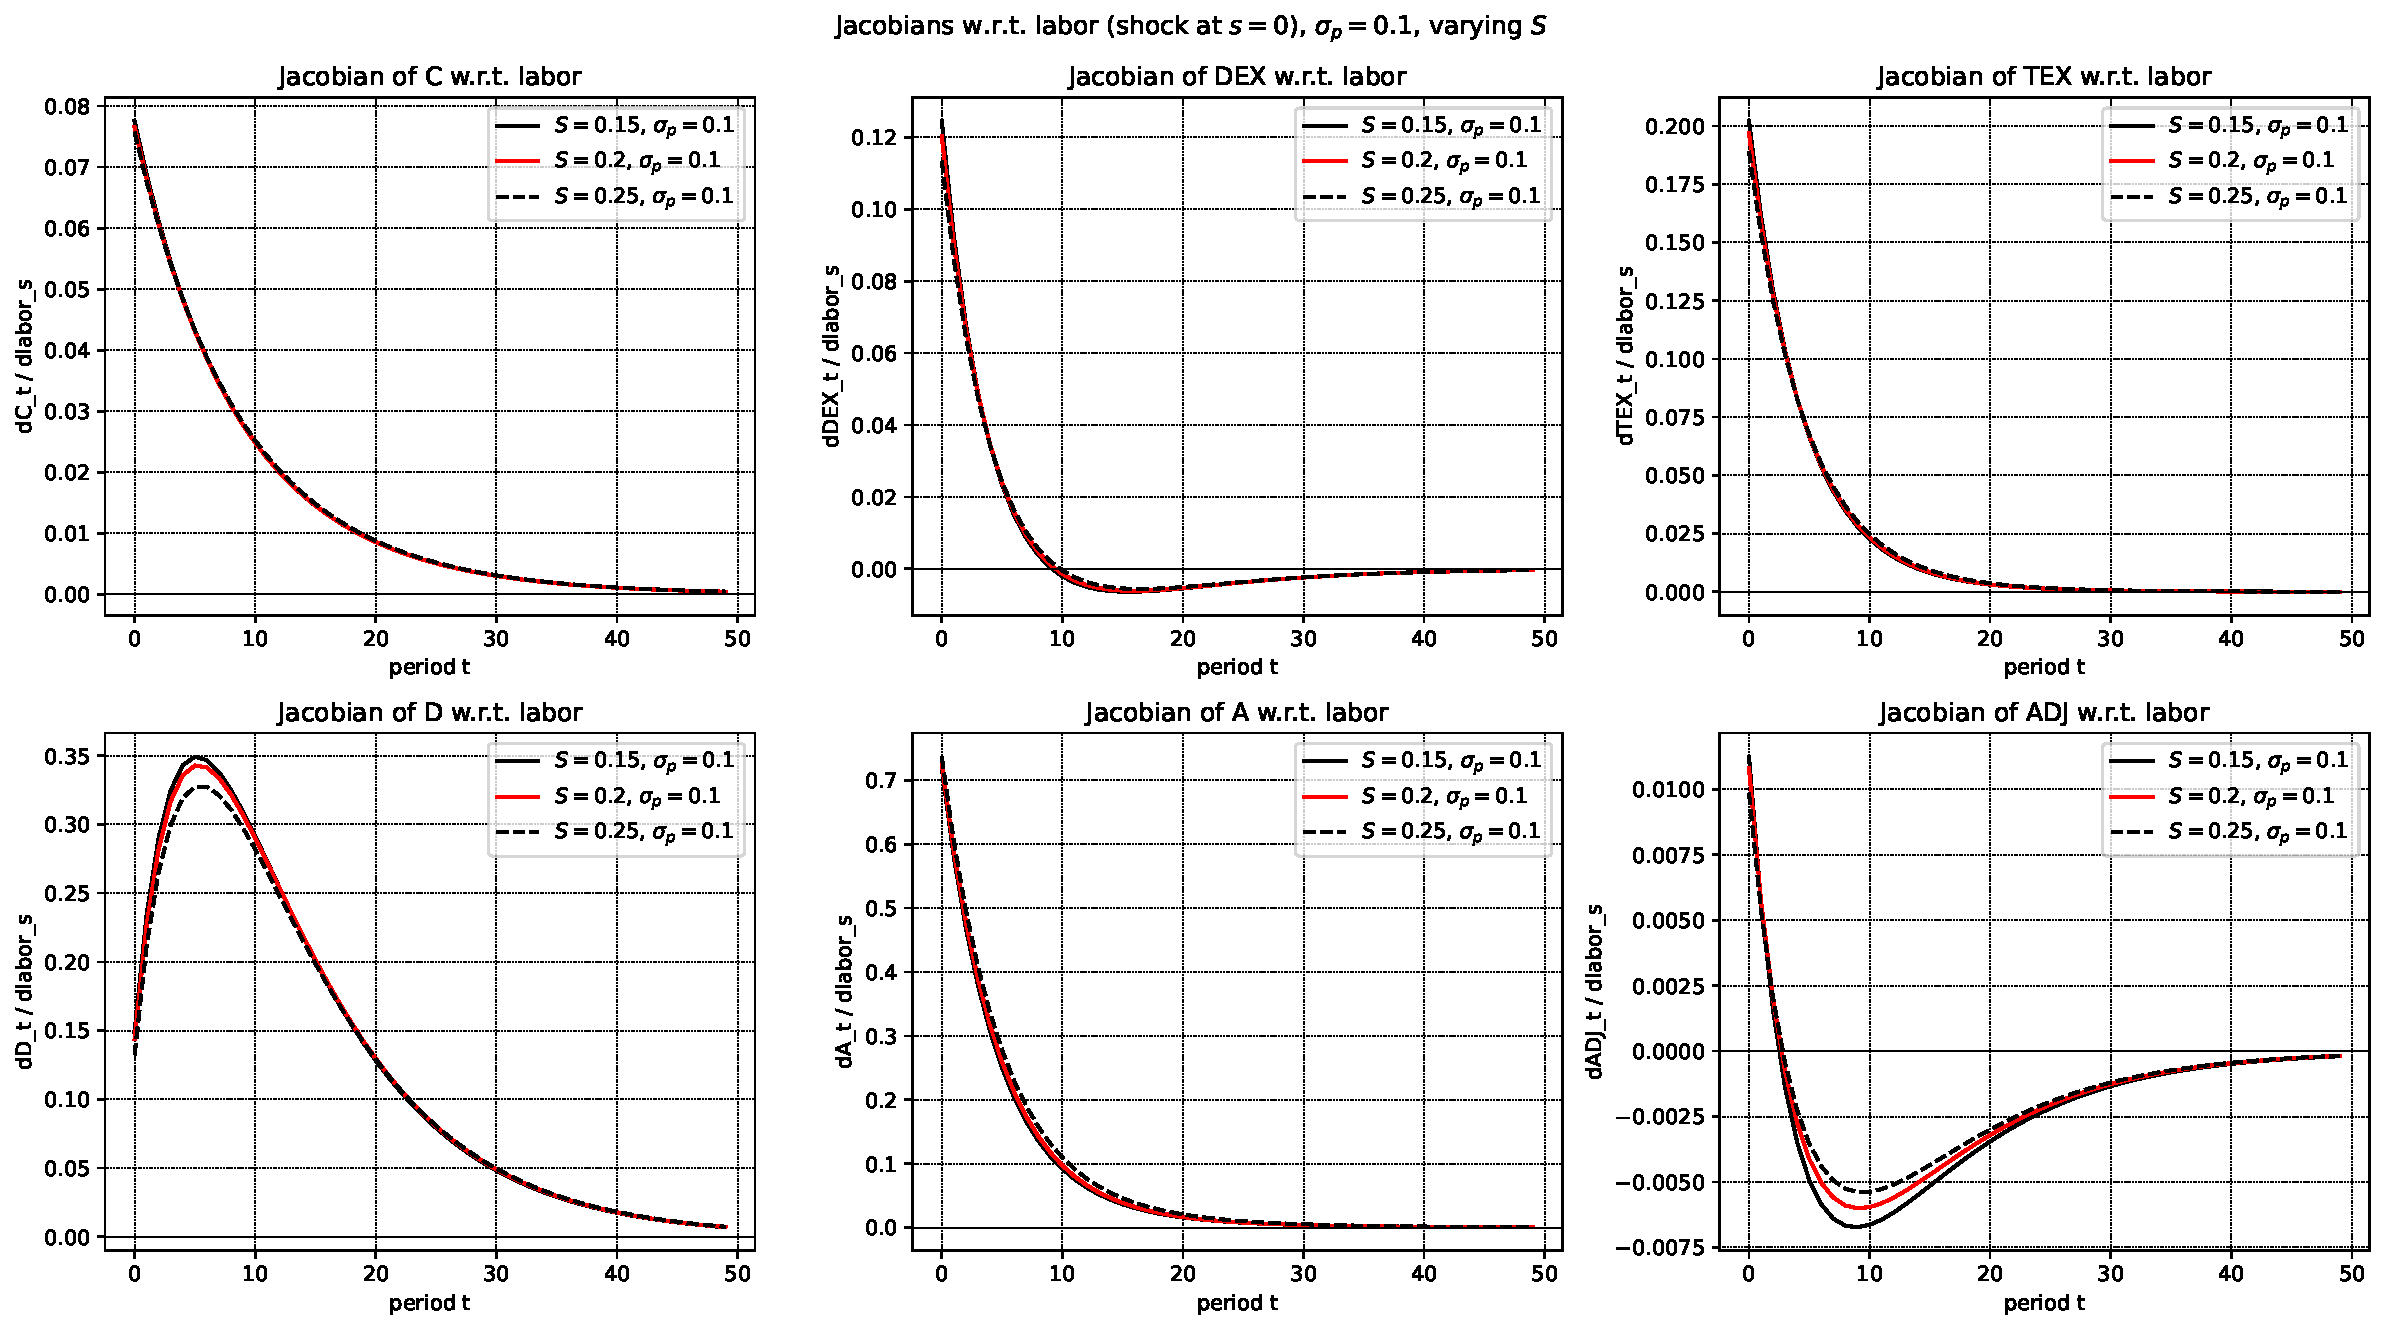
\includegraphics[width=0.78\linewidth]{Combined_varS_Inf_Jacobians_labor.pdf}
	\end{center}
	\vspace{0.25em}
	\begin{itemize}
		\item Varying $S$ (given $\sigma_p$): dynamics / \textbf{shape} of the Jacobian change
		\item The \textbf{impact} response remains essentially the same
	\end{itemize}
\end{frame}

\begin{frame}[label = Update2JacPrice]
	\frametitle{Jacobians: prices change shape, MPC stays the same}
	\begin{center}
		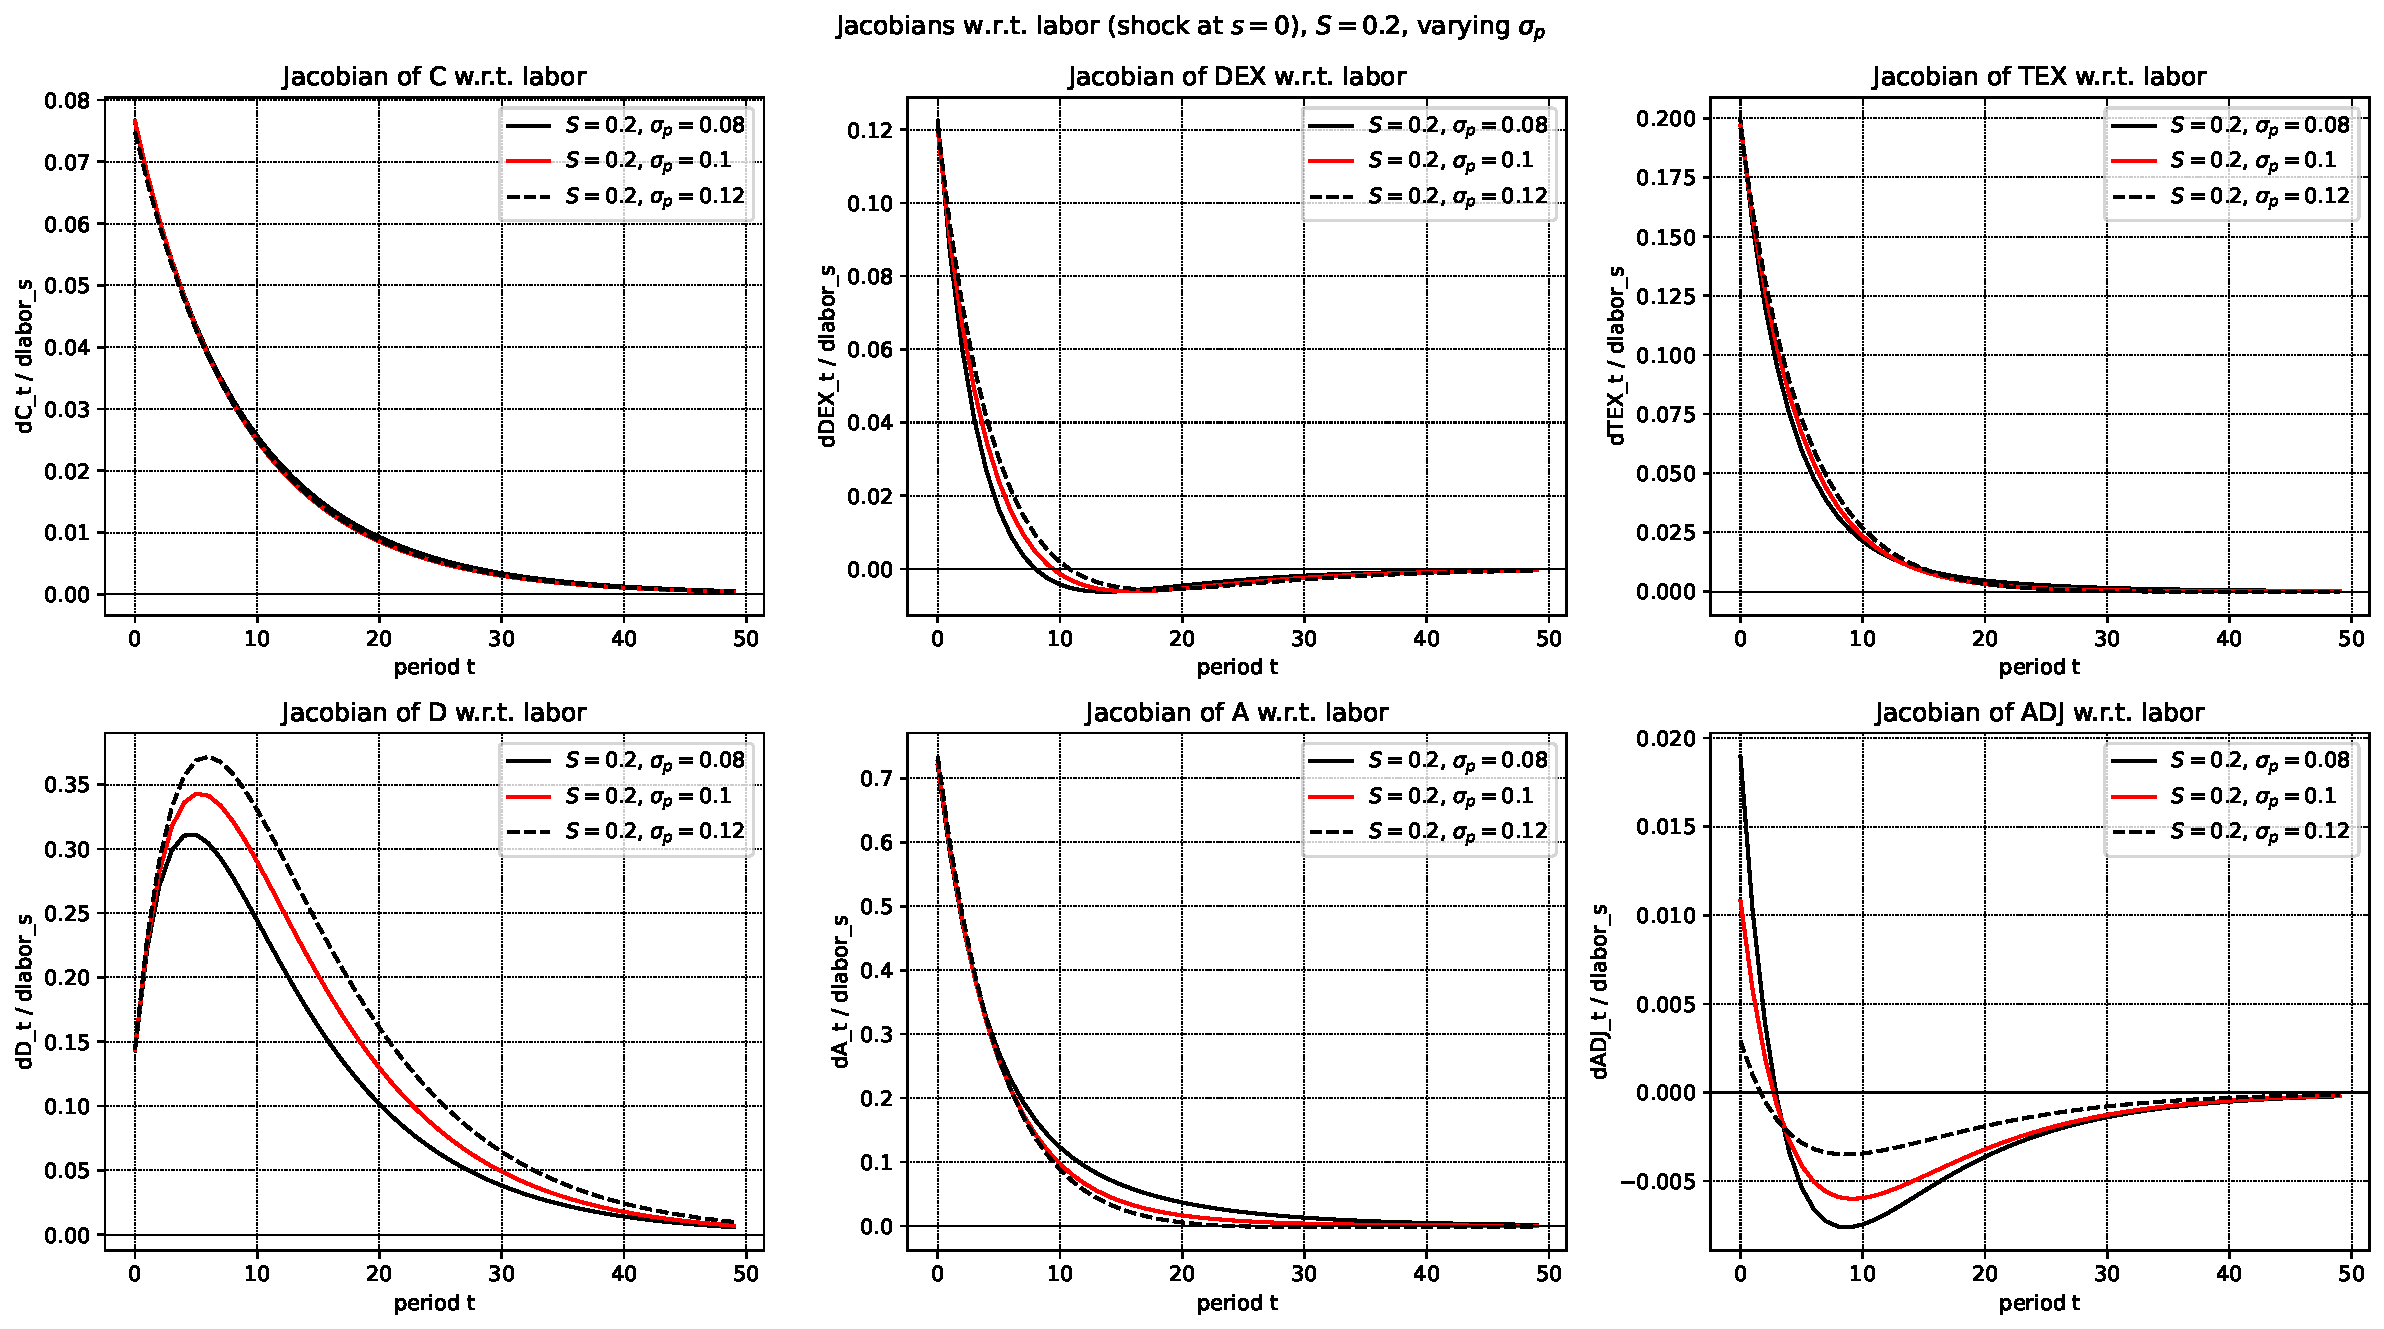
\includegraphics[width=0.78\linewidth]{Combined_varP_Inf_Jacobians_labor.pdf}
	\end{center}
	\vspace{0.25em}
	\begin{itemize}
		\item Varying $\sigma_p$ (given $S$): dynamics / \textbf{shape} of the Jacobian change
		\item The \textbf{impact} response remains essentially the same
	\end{itemize}
\end{frame}


%============================================================
\section{Open questions}
%============================================================

%%% Open questions:
% Main focus:   change to Sarch and price vs compare different smoothing mechanisms all together
%               Either add exogeneous switching probability also to durablemodel or delete this from Retirement
\begin{frame}[label = OpenFocus]
	\frametitle{Open question: what is the main focus?}
	\begin{enumerate}\setlength\itemsep{1.1em}
		\item \textbf{Search + price as alternative to EV taste shocks}
        \begin{itemize}
            \item Need to compare with EV taste shock (not lognormal one)
            \item Drop exogenous switch option in retirement problem
            \item[$\implies$] Narrow and targeted focus with clear punchline
        \end{itemize}
		\item \textbf{Compare all smoothing mechanisms side by side}
        \begin{itemize}
            \item Add exogeneous switch probability and log-normal taste shocks in durable model
            \item[$\implies$] Broader focus and more systematic review
        \end{itemize}
	\end{enumerate}
\end{frame}

%% Theory: Could add mathematical proofs about smoothing (with Akshay?)
\begin{frame}[label = OpenTheory]
	\frametitle{Open question: Add mathematical proofs}
    \begin{itemize}\setlength\itemsep{0.9em}
        \item Prove that search / prices / taste remove EGM non-monotonicities
        \item work with Akshay on formal results (cannot fact-check Claude by myself)
    \end{itemize}
\end{frame}

%% Open to-dos
\begin{frame}[label = Todo]
	\frametitle{Other: To-dos}
	\begin{itemize}\setlength\itemsep{0.9em}
		\item Comparison metric: no of kinks, euler errors, convergence no of iterations, solution time
		\item Estimation/calibration example of why opposite economic effects matter? Similar to Beraja and Zorzi
		\item Micro data for duration ($\implies$ search cost) and price dispersion
	\end{itemize}
\end{frame}
% \begin{frame}[label = Roadmap]
% 	\frametitle{Baseline roadmap for this updates deck}
% 	\begin{enumerate}\setlength\itemsep{0.85em}
% 		\item Lock previous story: search needs complements; taste shifts $c$ the other way
% 		\item Highlight Update~1: search + price dispersion
% 		\item Highlight Update~2: durables --- common policy shifts, divergent SS / Jacobians
% 		\item Resolve open questions: focus, role of exogenous $p$, theory proofs
% 	\end{enumerate}
% \end{frame}

% \begin{frame}[plain]
% 	\centering
% 	\vspace{2.5em}
% 	{\LARGE Thank you}\\[1.5em]
% 	{\large Repo: \url{https://github.com/AMonninger/DCEGM_Search}}
% \end{frame}

\end{document}
